\subsection{Rewording at scale: machine paraphrases of 700 real tasks}
\label{sec:paraphrase}

Our other tests of rewording rest on the development rewordings (five tasks) or on
damage made by a program (Section~\ref{sec:edits}). Here the rewordings come from neither. We took
the \WidenTasksAll{} definitions of Section~\ref{sec:many} and paraphrased each one by machine: back-translation
from English into German and back, and into French and back, sentence by sentence, with MarianMT
models \citep{junczys2018marian,tiedemann2020opusmt} and beam search without sampling. On average
\WidenKeptDe{}\% (German) and \WidenKeptFr{}\% (French) of the words of a definition survive; \WidenSameDe{}
German and \WidenSameFr{} French paraphrases equal the original. Two more pivots, Spanish and Italian, were made later, for the checks below (\WidenSpKept{}\% and \RerouteItKept{}\% of the words survive; \WidenSpSame{} and \RerouteItSame{} paraphrases equal the original). Two more pivots, Spanish and Italian, were made later, for the checks below (\WidenSpKept{}\% and \RerouteItKept{}\% of the words survive; \WidenSpSame{} and \RerouteItSame{} paraphrases equal the original). They are used as they come, poor
ones included. A paraphrased input is an input of its task whose definition has been replaced by the
paraphrase. \WidenTasksCal{} of the tasks are kept for choosing and calibrating (they are not used
again), and \WidenTasksEval{} are used for evaluation, arriving in a random order, each with its
zone. No model is trained; the test is about routes, with the T5-base word-vectors and the rule of
Section~\ref{sec:method} unchanged.

\paragraph{Measures.} All are shares. \textsf{C}: tasks that arrive with at least one unedited input inside an
older zone. \textsf{U}: unedited inputs given to their own task. \textsf{P}: paraphrased inputs that lie inside their
own task's zone and are given to it, a correct certificate. \textsf{M}: paraphrased inputs that are certified
for \emph{another} task, a wrong certificate: the answer is stable, but it comes from the wrong
adapters. \textsf{R}: paraphrased inputs given to their own task, with or without a certificate. These letters name measures in this section and its appendix only; they are not the covariance, the radius or the zone of the method.

\paragraph{The result for \cert{}.} With \WidenParaInputs{} paraphrased inputs (German and
French pivot together) we find \textsf{C}~=~\WidenRefTfiveC{}\%, \textsf{U}~=~\WidenRefTfiveU{}\%, \textsf{P}~=~\WidenRefTfiveP{}\%,
\textsf{M}~=~\WidenRefTfiveM{}\% and \textsf{R}~=~\WidenRefTfiveR{}\%. By pivot, \textsf{P} is \WidenRefTfiveFrP{}\% (French),
\WidenRefTfiveDeP{}\% (German) and \WidenRefTfiveEsP{}\% (Spanish); \textsf{M} is \WidenRefTfiveFrM{}\%,
\WidenRefTfiveDeM{}\% and \WidenRefTfiveEsM{}\%; \textsf{R} is \WidenRefTfiveFrR{}\%, \WidenRefTfiveDeR{}\% and
\WidenRefTfiveEsR{}\%. The Spanish paraphrases were made later, for the check described below, and the Italian ones last, for the fallback tests (on the Italian pivot \textsf{P}~=~\WidenRefTfiveItP{}\%, \textsf{M}~=~\WidenRefTfiveItM{}\%,
\textsf{R}~=~\WidenRefTfiveItR{}\%, inside the same ranges); \cert{} was not tuned on any of the four. So between four and five in ten machine-paraphrased inputs get a correct certificate
(\WidenRefTfivePLow{}\% to \WidenRefTfivePHigh{}\%, depending on the language the paraphrase went through), \WidenRefTfiveMLow{}\% to
\WidenRefTfiveMHigh{}\% are certified for another task, and the rest are uncertified. About three quarters of all paraphrased inputs (\WidenRefTfiveRLow{}\% to \WidenRefTfiveRHigh{}\%) reach their own task, with or
without a certificate. The figures of \FiveCertRightLight{}\%, \FiveCertRightMedium{}\% and
\FiveCertRightHeavy{}\% of Section~\ref{sec:reworded} were measured on five tasks that are far apart and on the development
rewordings. This is a limitation of the method as built: the zones are narrow at scale.

\paragraph{Can the zones be made wider?} We tried five ways, each with a rule for success written
before the run (Appendix~\ref{app:widen}): (1) the hidden states of a frozen causal language model
instead of the word-vectors; (2) a metric that counts distance in units of what paraphrasing does;
(3) a frozen sentence encoder of 22 million weights \citep{reimers2019sbert,wang2020minilm} with
a radius set by split-conformal calibration; (4) a zone decided by a frozen inference model
\citep{he2023debertav3} that judges whether two instructions ask for the same thing; (5) the same kind of judge, asked sentence by sentence. None of the five met the bar set for it in advance
(Table~\ref{tab:widenmain}, Figure~\ref{fig:widen}). For (3) to (5) the bar was \textsf{P}~$\ge$~75\%, \textsf{M}~$\le$~5\% and \textsf{C}~$\le$~19\%, read on the French pivot for (3) and (4) and on the Italian pivot for (5); the encoder reached \textsf{P}~=~\WidenEncPrimP{}\%,
\textsf{M}~=~\WidenEncPrimM{}\% and \textsf{C}~=~\WidenEncPrimC{}\%, the judge \textsf{P}~=~\WidenJudgeFrP{}\%,
\textsf{M}~=~\WidenJudgeFrM{}\% and \textsf{C}~=~\WidenJudgeC{}\%; (5) reached, on the Italian pivot that no study had read, \textsf{P}~=~\WidenSentItP{}\%, \textsf{M}~=~\WidenSentItM{}\% and \textsf{C}~=~\WidenSentC{}\%, the best point so far: \textsf{P} and \textsf{C} are on the right side of the success lines, \textsf{M} is above the 9\% limit.

\begin{table}[t]
  \caption{Machine paraphrases of 700 real tasks, routes only: \cert{} and the
  attempts to widen the zones, each in the setting named before its run. \textsf{C}: tasks that collide;
  \textsf{P}: paraphrased inputs certified for their own task; \textsf{M}: certified for another task; \textsf{R}: given to
  their own task; all in \%. ``Both'': German and French pivot together. Paper: T5-base word-vectors, weighted mean,
  $\kappa = 0.5$; its second row is the French pivot alone, the reference for the rows (2) to (4), which are French. (1) was run with another model, SmolLM2-135M, so it has its own reference row; the
  hidden state is that of the last layer, with one radius for all tasks. (2) uses the T5-base word-vectors with a metric fitted on
  paraphrases, read at the radius where \textsf{C} equals that of \cert{}, which is why its \textsf{C} is the same.
  (3) is MiniLM-L6 with the paraphrase ruler and a split-conformal radius ($\alpha = 0.1$); (4) is a MiniLM filter and the
  DeBERTa-v3-xsmall inference model ($\tau = \WidenJudgeTau{}$); (5) the same judge, sentence by sentence, read on the Italian pivot (its French-pivot point is in Figure~\ref{fig:widen}). Settings other than these are in
  Appendix~\ref{app:widen}. Units: rows marked ``both'' use \WidenParaInputs{} paraphrased inputs, the French rows \WidenParaInputsPivot{}, except (4) and (5), which
  take the instruction as a separate field and count one paraphrased instruction per task (\WidenTasksEval{}); its \textsf{C} is about the tasks' original
  instructions. The pre-registered reference of (2) is the old ruler at the same radius (\textsf{P} \WidenRulerTfivePOld{}\%, \textsf{M} \WidenRulerTfiveMOld{}\%).}
  \label{tab:widenmain}
  \centering
  \footnotesize
  \setlength{\tabcolsep}{3pt}
  \begin{tabular}{llcrrrrl}
    \toprule
    & Features and zone & Pivot & \textsf{C} & \textsf{P} & \textsf{M} & \textsf{R} & Verdict \\
    \midrule
    Paper & T5-base word-vectors, weighted mean & both & 16.9 & 40.5 & 7.6 & 75.4 & reference \\
    Paper & T5-base word-vectors, weighted mean & French & 16.9 & 39.8 & 9.2 & 75.4 & ref. for (2)--(4) \\
    \midrule
    (1) & SmolLM2 word-vectors & both & 18.9 & 42.1 & 8.9 & 75.6 & ref. for (1) \\
    (1) & SmolLM2 last layer & both & 25.7 & 64.9 & 13.7 & 83.2 & against \\
    (2) & T5-base, paraphrase ruler & French & 16.9 & 42.0 & 10.7 & 84.4 & against \\
    (3) & MiniLM, ruler, $\alpha = 0.1$ & French & 16.6 & 71.2 & 11.6 & 86.1 & against \\
    (4) & MiniLM and NLI judge & French & 36.0 & 58.9 & 34.7 & 64.7 & against \\
    (5) & MiniLM, sentence-wise NLI judge & Italian & 12.4 & 76.1 & 10.9 & 88.7 & against \\
    \midrule
    Bar (3)--(5) & \multicolumn{2}{l}{fixed in advance} & $\le 19$ & $\ge 75$ & $\le 5$ & & \\
    \bottomrule
\end{tabular}

\end{table}

\begin{figure}[t]
  \centering
  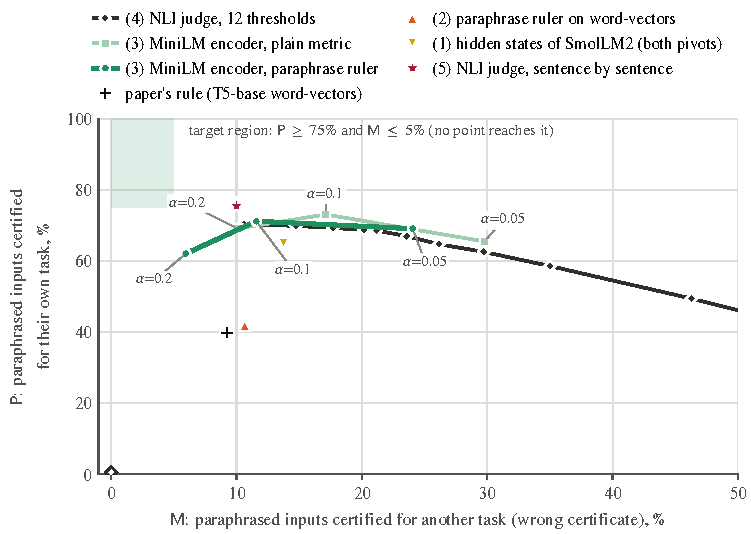
\includegraphics[width=0.86\linewidth]{figures/widen_tradeoff}
  \caption{Correct against wrong certificates on paraphrased inputs (French pivot; hidden states of
  (1): both pivots). The shaded box is the target. The sentence encoder (3) is shown plain and with
  the paraphrase ruler at $\alpha = 0.05, 0.1, 0.2$; the curve of the judge (4) has one point per
  threshold, and its point at the strictest threshold (open) covers almost nothing. One point
  of the curve (the loosest threshold) lies beyond the right edge. Only (3) at $\alpha = 0.1$ with the ruler, (4) at $\tau = \WidenJudgeTau{}$ and (5) were named before the runs; (5) is shown at its French-pivot value.}
  \label{fig:widen}
\end{figure}

\paragraph{What rises and what does not.} The sentence encoder lifts the share of correct certificates
from \WidenRefTfiveFrP{}\% (\cert{}, French pivot alone) to between \WidenEncRulerTwentyFrP{}\% and
\WidenEncPlainTenFrP{}\% over its six settings (Table~\ref{tab:widenencoder} in the appendix). At $\alpha = 0.1$ and
$0.2$ ($\alpha$ is the level of the split-conformal radius, not the scaling factor of the adapters) it gives between \WidenEncRHighLow{}\% and \WidenEncRHighHigh{}\% of the inputs to the right task, where \cert{}
gives \WidenRefTfiveFrR{}\%. The wrong certificates do not stay low as \textsf{P} rises. The setting with the fewest
(\textsf{M}~=~\WidenEncRulerTwentyFrM{}\%, above the bar of 5\%) has \textsf{P}~=~\WidenEncRulerTwentyFrP{}\%, and the setting with the
highest \textsf{P} (\WidenEncPlainTenFrP{}\%) has \textsf{M}~=~\WidenEncPlainTenFrM{}\%. \cert{} has \textsf{M}~=~\WidenRefTfiveFrM{}\%
on the French pivot alone, so the first setting is lower in \textsf{M} and higher in \textsf{P} than \cert{}; it was
not the primary setting, and we checked it on held-out paraphrases (next paragraph). Most of the tasks that collide under \cert{} are siblings
that differ in one or a few decisive words: a date format day-month against month-day, the closest integers against
the farthest, the reaction of a person in the ATOMIC tasks against their intent
(Table~\ref{tab:widensiblings} in the appendix, a selection). Every feature for which we inspected the collisions puts the
rewordings of such siblings together. The judge also certifies some paraphrases for unrelated tasks, for example
sentence generation from a relation for an entailment task. The judge is good on single pairs (area under the curve
\WidenJudgeAucNli{} on calibration pairs) and bad as a zone: a text is judged against up to \WidenJudgeLimit{} nearby
instructions, and one wrong ``same'' from an older zone, or from any zone when its own zone does not hold it, is enough.

\paragraph{One setting, checked on held-out paraphrases.} After the runs we saw that one setting of the sentence
encoder that was not the primary one (paraphrase ruler, $\alpha = 0.2$) was ahead of \cert{} on the French pivot
on each measure. A comparison chosen after the results proves nothing, so we fixed one more check before running it: the same two
rules on paraphrases made through Spanish, which no study had read, on the same \WidenTasksEval{} tasks, with nothing fitted again.
It would count as confirmed if the encoder setting gained at least \WidenSpAskP{} points in \textsf{P} and \WidenSpAskR{} points in \textsf{R}
and had no more wrong certificates. On the Spanish pivot (Table~\ref{tab:widenspanish}) \cert{} has
\textsf{P}~=~\WidenRefTfiveEsP{}\%, \textsf{M}~=~\WidenRefTfiveEsM{}\% and \textsf{R}~=~\WidenRefTfiveEsR{}\%, the encoder setting \textsf{P}~=~\WidenSpEncEsP{}\%,
\textsf{M}~=~\WidenSpEncEsM{}\% and \textsf{R}~=~\WidenSpEncEsR{}\%. The gain in \textsf{P} is \WidenSpGainP{} points, so by our rule the check is \emph{not
confirmed} (the gain in \textsf{R}, \WidenSpGainR{} points, and \textsf{M} pass). On this split the encoder setting is ahead on each measure, but by less than we
asked for; \cert{} itself does better on these paraphrases, which keep more of the original words
(\WidenSpKept{}\% against \WidenKeptDe{}\% and \WidenKeptFr{}\%). On \WidenSplitCount{} other random splits of the tasks into calibration and
evaluation tasks (everything fitted again), the Spanish pivot gives \textsf{P} of \WidenSplitRulePMean{}\% (\WidenSplitRulePLow{} to
\WidenSplitRulePHigh{}) and \textsf{M} of \WidenSplitRuleMMean{}\% (\WidenSplitRuleMLow{} to \WidenSplitRuleMHigh{}) for \cert{}, and
\textsf{P} of \WidenSplitEncPMean{}\% (\WidenSplitEncPLow{} to \WidenSplitEncPHigh{}) and \textsf{M} of \WidenSplitEncMMean{}\%
(\WidenSplitEncMLow{} to \WidenSplitEncMHigh{}) for the encoder setting, which therefore depends more on the split. On \WidenSplitMoreM{} of these \WidenSplitCount{} splits the encoder setting has more wrong
certificates than \cert{} (and on \WidenSplitMoreC{} of them more collisions), so the advantage on every measure is a property
of the original split, not of the setting. We report the encoder
zone as a variant, not as an improvement that we have shown. It needs a second model, run at several prefix lengths, for every input
(\WidenEncMs{} ms per input on two CPU threads), it has no edit bound, its radius does not keep the promised coverage on another pivot (\textsf{Z} is
\WidenSpEncEsZ{}\% on Spanish and \WidenSpEncFrZ{}\% on French where \WidenSpPromise{}\% was promised, and \WidenSpEncDeZ{}\% on the German pivot it
was fitted on), and with it none of the medium and heavy development rewordings of the five benchmark tasks lies inside a zone
(\WidenSpBenchMediumZone{}\% and \WidenSpBenchHeavyZone{}\%); they are still given to the right task.

\begin{table}[t]
  \caption{The check on Spanish-pivot paraphrases: \cert{} and the encoder setting (paraphrase ruler,
  $\alpha = 0.2$) on the three pivots, \WidenSpInputs{} paraphrased inputs each; nothing was fitted again for Spanish. ``Encoder'': the sentence encoder with the paraphrase ruler at $\alpha = 0.2$. In \%.}
  \label{tab:widenspanish}
  \centering
  \footnotesize
  \setlength{\tabcolsep}{3pt}
  \begin{tabular}{lrrrrrrrrrr}
    \toprule
    & & \multicolumn{3}{c}{French} & \multicolumn{3}{c}{German} & \multicolumn{3}{c}{Spanish} \\
    \cmidrule(lr){3-5} \cmidrule(lr){6-8} \cmidrule(lr){9-11}
    & \textsf{C} & \textsf{P} & \textsf{M} & \textsf{R} & \textsf{P} & \textsf{M} & \textsf{R} & \textsf{P} & \textsf{M} & \textsf{R} \\
    \midrule
    Paper's rule & 16.9 & 39.8 & 9.2 & 75.4 & 41.2 & 5.9 & 75.5 & 50.4 & 9.7 & 77.5 \\
    Encoder & 12.1 & 62.1 & 6.0 & 90.0 & 72.6 & 8.1 & 89.7 & 63.8 & 5.3 & 91.7 \\
    \bottomrule
\end{tabular}

\end{table}

\begin{table}[t]
  \caption{The same two rules on \WidenSplitCount{} other random splits of the \WidenTasksAll{} tasks, Spanish pivot: mean (smallest to largest), with
  ruler and radius fitted again on each split. In \%.}
  \label{tab:widensplits}
  \centering
  \footnotesize
  \begin{tabular}{lcc}
    \toprule
    Spanish pivot & Paper's rule & Encoder \\
    \midrule
    Tasks that collide (\textsf{C}), \% $\downarrow$ & 16.0 (14.3 to 17.3) & 12.7 (9.1 to 16.6) \\
    Right certificate (\textsf{P}), \% $\uparrow$ & 49.4 (48.3 to 50.7) & 63.1 (55.5 to 70.0) \\
    Wrong certificate (\textsf{M}), \% $\downarrow$ & 7.9 (4.2 to 10.4) & 6.0 (2.4 to 9.7) \\
    Sent to own task (\textsf{R}), \% $\uparrow$ & 76.9 (75.8 to 78.1) & 90.4 (87.7 to 93.3) \\
    \bottomrule
\end{tabular}

\end{table}

\paragraph{Do later tasks re-route reworded inputs?} The stress test of Section~\ref{sec:stress} built by hand a case in which a best-match rule
changes an old route. With the paraphrased inputs we can count how often this happens among real tasks. For every paraphrased input we compare its route
right after its own task has arrived with its route after all \WidenTasksEval{} tasks. The reading was fixed before the run (Appendix~\ref{app:reroute}): the zones
add something at scale if \nearest{} changes at least 5\% of the routes and \cert{} at most half as many, and little if \nearest{} changes fewer than \RerouteLimitLow{}\%.

The result is against us (Table~\ref{tab:reroute}); by the reading fixed in advance, ``the zones add little here''. \nearest{} changed \RerouteNearNChanged{} of \RerouteInputs{} routes (\RerouteNearChanged{}\%), and \cert{} changed the same
\RerouteCertNChanged{}, all of them outside every zone. None of the \RerouteCertInZone{}\% of the inputs that were inside a zone at arrival changed, as Theorem~\ref{thm:writeonce} says, but
the nearest-zone rule did not change them either. We had expected \RerouteExpectNearLow{}\% to \RerouteExpectNearHigh{}\% for \nearest{}; that expectation was wrong. In this collection the certified switch adds
the proof, and no stability that we could measure.

\begin{table}[t]
  \caption{Do later tasks re-route reworded inputs? Routes only; \WidenTasksEval{} real tasks. ``Own'': share of the \RerouteInputs{} paraphrased inputs (French and German pivot) given to their own task after all tasks; ``Italian: own'':
  the same on the \RerouteInputsPivot{} Italian-pivot inputs (paraphrases made for the two fallback tests and read only for them). ``Changed'': route after all tasks differs from the route right after the input's own task arrived. ``In a zone'': inside a zone
  at arrival. ``Unedited'': unedited inputs given to their own task at the end (none changed under any rule). \signature{}: nearest signature in plain distance, no radius. \hybrid{}: the oldest zone that holds the
  input, else the nearest signature in plain distance. \scaled{}: nearest signature, its distance divided by the distance of the task's signature to the nearest signature of the unrelated tasks. \certscaled{}: the oldest zone that holds the input, else \scaled{}.
  \hybrid{} was designed after the first three results were seen and \scaled{} after \hybrid{}, on the same data; none has a free setting.}
  \label{tab:reroute}
  \centering
  \scriptsize
  \setlength{\tabcolsep}{2pt}
  \begin{tabular}{lrrrrr}
    \toprule
    Rule & \shortstack[r]{Sent to own\\task, \% $\uparrow$} & \shortstack[r]{Italian pivot: sent\\to own task, \% $\uparrow$} & \shortstack[r]{Routes changed,\\\% (n) $\downarrow$} & \shortstack[r]{Inside a zone\\at arrival, \%} & \shortstack[r]{Unedited, sent to\\own task, \% $\uparrow$} \\
    \midrule
    \signature{} (plain nearest signature) & 91.3 & 93.1 & 2.22 (93) & -- & 98.4 \\
    \nearest{} (nearest zone) & 75.4 & 77.0 & 0.31 (13) & -- & 98.4 \\
    \cert{} (the rule of the paper) & 75.4 & 76.8 & 0.31 (13) & 48.1 & 83.1 \\
    \hybrid{} (zones, then nearest signature) & 85.6 & 88.5 & 1.95 (82) & 48.1 & 83.1 \\
    \scaled{} (scaled by the distance to unrelated text) & 94.4 & 95.9 & 1.60 (67) & -- & 98.4 \\
    \certscaled{} (zones, then \scaled{}) & 88.6 & 91.3 & 1.33 (56) & 48.1 & 83.1 \\
    \bottomrule
\end{tabular}

\end{table}

\begin{table}[t]
  \caption{The same rules on the benchmark tasks with the development rewordings (routes only): share of the \RerouteBenchInputs{} inputs given to their own task after the last task; ``(n)'': routes changed by later tasks (of \RerouteBenchInputs{}, including the inputs of the last task, which cannot change).
  With the original and the light wording every rule gives 100\% and changes nothing.}
  \label{tab:reroutebench}
  \centering
  \footnotesize
  \setlength{\tabcolsep}{3pt}
  \begin{tabular}{lrrrr}
    \toprule
    & \multicolumn{2}{c}{Five tasks} & \multicolumn{2}{c}{Fifteen tasks} \\
    \cmidrule(lr){2-3} \cmidrule(lr){4-5}
    Rule & \shortstack[r]{Medium wording:\\own task, \% $\uparrow$\\(routes changed)} & \shortstack[r]{Heavy wording:\\own task, \% $\uparrow$\\(routes changed)} & \shortstack[r]{Medium wording:\\own task, \% $\uparrow$\\(routes changed)} & \shortstack[r]{Heavy wording:\\own task, \% $\uparrow$\\(routes changed)} \\
    \midrule
    \signature{} & 76.8 (55) & 60.0 (100) & 71.6 (74) & 60.0 (100) \\
    \nearest{} & 100.0 (0) & 93.8 (0) & 100.0 (0) & 93.8 (0) \\
    \cert{} & 100.0 (0) & 93.8 (0) & 100.0 (0) & 93.8 (0) \\
    \hybrid{} & 76.8 (55) & 60.0 (100) & 71.6 (74) & 60.0 (100) \\
    \scaled{} & 100.0 (0) & 93.8 (0) & 100.0 (0) & 93.8 (0) \\
    \certscaled{} & 100.0 (0) & 93.8 (0) & 100.0 (0) & 93.8 (0) \\
    \bottomrule
\end{tabular}

\end{table}

Two more rules were computed on the same routes after this result, each written down before it was computed. The plain nearest signature, without radii, is the usual prototype rule. It changed
\RerouteSigNChanged{} routes (\RerouteSigChanged{}\%), and \RerouteSigNLost{} inputs lost their own task; by its reading fixed in advance that is ``some'' re-routing, less than the 5\% we had expected.
But it gave \RerouteSigOwnEnd{}\% of the paraphrased inputs to their own task, where \cert{} and \nearest{} give \RerouteCertOwnEnd{}\% (Spanish pivot: \RerouteSigEsOwn{}\% against \RerouteCertEsOwn{}\% for \cert{} and \RerouteNearEsOwn{}\% for \nearest{}; unedited inputs:
\RerouteSigUnOwn{}\% against \RerouteCertUnOwn{}\%). At this scale the simplest rule serves reworded inputs better than \cert{}, and it pays with about two silent changes in a hundred inputs. Dividing the distance by the radius is the fallback that
we chose on the benchmark tasks; it keeps routes stable here and gives fewer inputs to their own task.

Zones first and the plain nearest signature outside them (\hybrid{}, designed after the result of the plain nearest signature was seen, on the same data, with no free setting) keeps every certificate and gives \RerouteHybOwnEnd{}\% of the inputs to their own task, with \RerouteHybChanged{}\% changed routes. It is not a repair. On the benchmark tasks with
the development rewordings the plain fallback is much worse than the fallback of \cert{}: \RerouteHybBenchFiveHeavyOwn{}\% against \RerouteCertBenchFiveHeavyOwn{}\% under the heavy rewording, and \RerouteHybBenchFiveHeavyChanged{} of the \RerouteBenchChangeable{} routes
that later tasks could change are changed by them. The two fallbacks trade places between the two tests.

A reading of why, from the numbers and not a test of its own: the radius of a zone is half the distance to the nearest known signature, and ``known'' means the unrelated tasks \emph{and} the earlier tasks. Write $U_k$ for the distance from the signature of task $k$ to the nearest
signature of the unrelated tasks only. On the benchmark tasks the radius is half of $U_k$ for all five tasks and for \RerouteBBenchFifteenCount{} of the fifteen; among the \WidenTasksEval{} real tasks it is so for only \RerouteBShare{}\% of them. For the others an earlier task, usually a
sibling, is nearer than every unrelated one; the radius of the newer sibling is then tiny, and its reworded inputs look far from it and are turned away by the nearest-zone fallback.

We then tested two fallbacks, each with its rule fixed before the run and with the verdict at scale read on paraphrases through a fourth language, Italian, that no study had read (Appendix~\ref{app:reroute}). Success meant at least \RerouteLineHeavy{}\% of the inputs to their own task under
heavy and \RerouteLineMedium{}\% under medium rewording on the benchmark tasks (five and fifteen), and at least \RerouteLineItalian{}\% on the Italian pivot; heavy rewording below \RerouteLineHeavyAgainst{}\% or the Italian pivot below \RerouteLineItalianAgainst{}\% counted against. A fallback scaled by the length of the opening
\emph{failed}: \RerouteNormHeavyFive{}\% under heavy rewording on the benchmark, although it gave \RerouteNormItOwn{}\% on the Italian pivot. A fallback scaled by $U_k$ alone, \scaled{}, \emph{succeeded} (Tables~\ref{tab:reroute} and~\ref{tab:reroutebench}): \RerouteBgHeavyFive{}\% under heavy and \RerouteBgMediumFive{}\% under medium rewording on the benchmark, as
the fallback of \cert{}, and \RerouteBgItOwn{}\% of the Italian-pivot inputs to their own task (plain nearest signature \RerouteSigItOwn{}\%, nearest zone \RerouteNearItOwn{}\%), \RerouteBgOwnEnd{}\% on the French and German pivot. With the zones of \cert{} in front (\certscaled{}: the same zones, the same certificates, the same theorem) it gives
\RerouteCertFourItOwn{}\% on the Italian pivot and \RerouteCertFourOwnEnd{}\% on the French and German pivot, where \cert{} gives \RerouteCertItOwn{}\% and \RerouteCertOwnEnd{}\%, and on the benchmark the routes and shares are those of \cert{}.

It has costs. After their task has arrived \RerouteCertFourChanged{}\% to \RerouteBgChanged{}\% of the paraphrased inputs change their route (French and German pivot; \RerouteBgItChanged{}\% on the Italian and \RerouteCertFourEsChanged{}\% to \RerouteBgEsChanged{}\% on the Spanish pivot; \RerouteCertChanged{}\% with the fallback of \cert{}). In the stress test of Section~\ref{sec:stress} a look-alike task takes uncertified old inputs that the fallback of \cert{} kept: with the light rewording as its definition \RerouteStressCertFourMedium{} of \RerouteStressOld{} with the medium and \RerouteStressCertFourHeavy{} with the heavy wording (0 and 0 for the fallback of \cert{}), and with the medium rewording as its definition \RerouteStressMedCertFourHeavy{} of \RerouteStressOld{} with the heavy wording (\RerouteStressMedCertHeavy{} for the fallback of \cert{}); no certified input changes. Its status: a variant found at the end of this work. The benchmark rewordings are the development set, so on that side it is no independent test;
no GPU run was repeated with it, but an input-by-input check on the benchmark sequences found its routes identical to those of \cert{} at every point where a score is taken. For the five-task sequence the radius is half of $U_k$ for all five tasks, so the two fallbacks order the tasks identically and the routes are the same by construction (the check finds \RerouteIdFiveLast{} differing routes in \RerouteIdFiveComparisons{} comparisons). For the fifteen-task sequence one task, \texttt{\RerouteIdTask{}} (the \RerouteIdTaskPos{}rd to arrive), has a radius that is half the distance to an earlier task and not half of $U_k$; even so \RerouteIdFifteenLast{} routes differ after the last task and \RerouteIdFifteenScored{} at any point from the arrival of the input's own task on, in every wording (they differ only at points before the input's own task has arrived, where no score is taken: \RerouteIdFifteenBeforeOriginal{}, \RerouteIdFifteenBeforeMedium{} and \RerouteIdFifteenBeforeHeavy{} inputs with the original, medium and heavy wording). Every score of the GPU runs of \cert{} and \nearest{} in this paper, for five and for fifteen tasks, is therefore also the score of the corresponding variant. The other route tests were not repeated with it (except the stress test), \cert{} remains the zone rule of every GPU run with instructions, and the certificates are the same under both. With this fallback the zones cost \RerouteZonesCost{} points of right routes on the Italian pivot, \RerouteZonesCostFG{} on the French and German pivot and \RerouteZonesCostEs{} on the Spanish pivot
compared with the best rule without zones (\RerouteBgItOwn{}\% against \RerouteCertFourItOwn{}\%, \RerouteBgOwnEnd{}\% against \RerouteCertFourOwnEnd{}\%), and give a proof for about half of the inputs (\RerouteCertInZone{}\% at arrival). None of these rules was run with trained answers.

\paragraph{The guarantee does not depend on the zone.} Theorem~\ref{thm:writeonce} needs only that the
zone of a task is a fixed set once the task has arrived and that membership is computed reproducibly from frozen parts
(Remark~\ref{rem:otherzones}); the proof does not use how the set was built. It therefore holds for every zone in this
section as defined; for the judge zone as measured, which judges only the \WidenJudgeLimit{} nearest tasks, see Appendix~\ref{app:widen}. What changes is how many inputs a zone covers, and for which task: a certificate promises a
stable answer, not the right task, and a certificate for the wrong task is a stable wrong routing.
The edit bound of Proposition~\ref{prop:edits} does not carry over, because it needs an average.

\paragraph{What this test is not.} Machine paraphrases are made by translation models, not by people.
There is one collection of tasks, in which many tasks are siblings, and the calibration and the
evaluation tasks come from it; the test uses one split and one order of arrival, except for the \WidenSplitCount{} extra splits of the Spanish check. The development rewordings of the five benchmark tasks
move further than a back-translation does: with the sentence encoder
\WidenEncBenchMediumZone{}\% (medium) and \WidenEncBenchHeavyZone{}\% (heavy) of them lie inside their own
zone, while all are still given to the right task. The settings that were not the primary ones
are observations made after the run, and none of them meets the bar.
